\documentclass{standalone}


% Copy of relevant parts from the main preamble.
\usepackage{mathtools}

% Uncomment the following to use Times New Roman and Cambria Math
% \usepackage{unicode-math}
% \unimathsetup{math-style=TeX}
% \setmathfont[range=\mathup/{num}]{Times New Roman}
% \setmathfont[range=\mathit/{greek,Greek,latin,Latin}]{Cambria Math}
% \setmathfont[range=\mathup/{greek,Greek,latin,Latin}]{Cambria Math}
% \setmathfont[range={"2212,"002B,"003D,"0028,"0029,"005B,"005D,"221A,
% "2211,"2248,"222B,"007C,"2026,"2202,"00D7,"0302,"2261,"0025,"22C5,
% "00B1,"2194,"21D4,"2032}]
% {Cambria Math}
% \setmainfont[Ligatures=TeX]{Times New Roman}

% Uncomment the following to use Linux Libertine
% \usepackage[libertine]{newtxmath}
% \usepackage[no-math]{fontspec}
% \setmainfont{Linux Libertine O}

% Uncomment the following to use TeX Gyre Termes
% \usepackage{unicode-math}
% \unimathsetup{math-style=TeX}
% \setmainfont{TeX Gyre Termes}
% \setmathfont{TeX Gyre Termes Math}

% Uncomment the following to use TeX Gyre Pagella
\usepackage{unicode-math}
\unimathsetup{math-style=TeX}
\setmainfont{TeX Gyre Pagella}
\setmathfont{TeX Gyre Pagella Math}

% \usepackage[sfmath]{kpfonts}
% \renewcommand*\familydefault{\sfdefault}
% \usepackage[T1]{fontenc}

% \usepackage[no-math]{fontspec}
% Always use Inconsolata
\setmonofont{Inconsolata}

\usepackage{microtype}


\usepackage[version=3]{mhchem}
\usepackage{chemfig}
\definesubmol\nobond{-[,0.2,,,draw=none]}
\setatomsep{2.25em}
\usetikzlibrary{positioning}
\tikzset{line join=bevel}

\begin{document}
    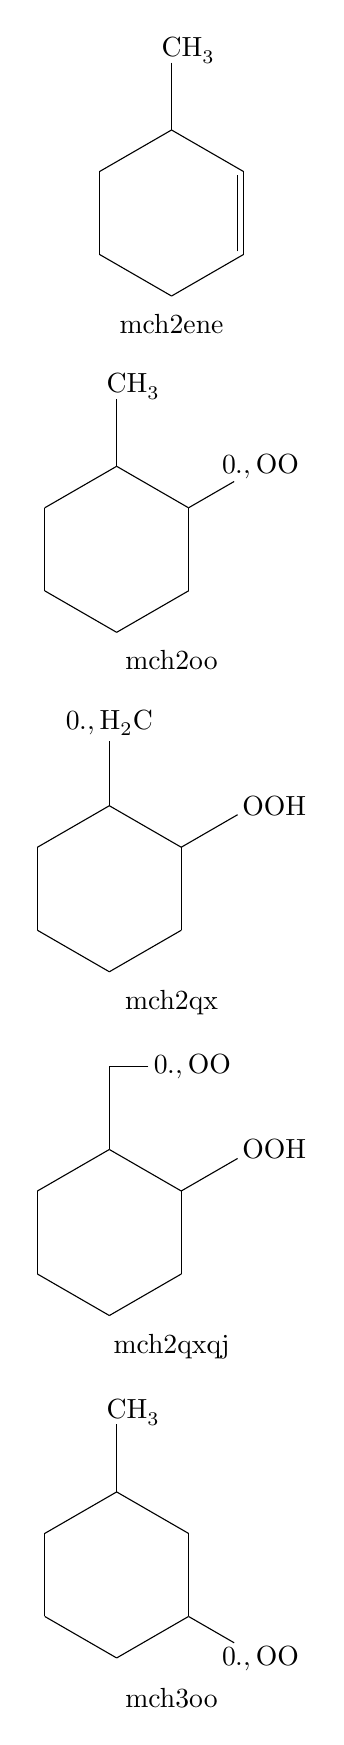
\begin{tikzpicture}[node distance=0.25cm]
        \node (mch2ene) {\chemname{\chemfig{CH_3-[6]*6(----=-)}}{mch2ene}};
        \node[below=of mch2ene] (mch2oo) {\chemname{\chemfig{CH_3-[6]*6(-----(-\lewis{0.,OO})-)}}{mch2oo}};
        \node[below=of mch2oo] (mch2qx) {\chemname{\chemfig{\lewis{0.,H_2C}-[6]*6(-----(-OOH)-)}}{mch2qx}};
        \node[below=of mch2qx] (mch2qxqj) {\chemname{\chemfig{\lewis{0.,OO}-[4]-[6]*6(-----(-OOH)-)}}{mch2qxqj}};
        \node[below=of mch2qxqj] (mch3oo) {\chemname{\chemfig{CH_3-[6]*6(----(-\lewis{0.,OO})--)}}{mch3oo}};
    \end{tikzpicture}
\end{document}
